% !TEX encoding = UTF-8 Unicode
\documentclass[margin,line]{res}
%\usepackage{helvetica} 
\usepackage{fontspec}
\setmainfont{Helvetica}[
  UprightFont = {*},
  BoldFont = {* Bold},
  SlantedFont = {* Oblique},
  BoldSlantedFont = {* Bold Oblique},
  ItalicFont=Helvetica Neue Italic,
  SmallCapsFont=Helvetica Neue LIght Italic]
%\usepackage{newtxsf}
\usepackage{xcolor}
\usepackage[hidelinks]{hyperref}
\usepackage{wrapfig,graphicx,lipsum}

\oddsidemargin -.7in %how far shifted left/right content is from left-hand side of page
\evensidemargin -.5in % ?
\textwidth=6.5in %how wide the main content (right) column is
\itemsep=0in % ?
\parsep=0in % ?
% TO CHANGE WIDTH OF SECTION HEADERS: open res.cls and change margin in line 445
% TO CHANGE TOP MARGIN OF PAGES: open res.cls and change margin in line 780 (\topmargin)
% TO CHANGE HEIGHT OF CONTENT: open res.cls and change margin in line 778 (\textheight)

\newenvironment{list1}{
  \begin{list}{$\bullet$}{
      \setlength{\itemsep}{0in}
      \setlength{\parsep}{0in} \setlength{\parskip}{0in}
      \setlength{\topsep}{0in} \setlength{\partopsep}{0in} 
      \setlength{\leftmargin}{0.17in}}}{\end{list}} % ?

\begin{document}

\name{\vspace*{-0.28in} \Large Mallory A Freeberg, PhD} %Change to move name up/down

%\begin{figure}[h!]
%    \flushright
%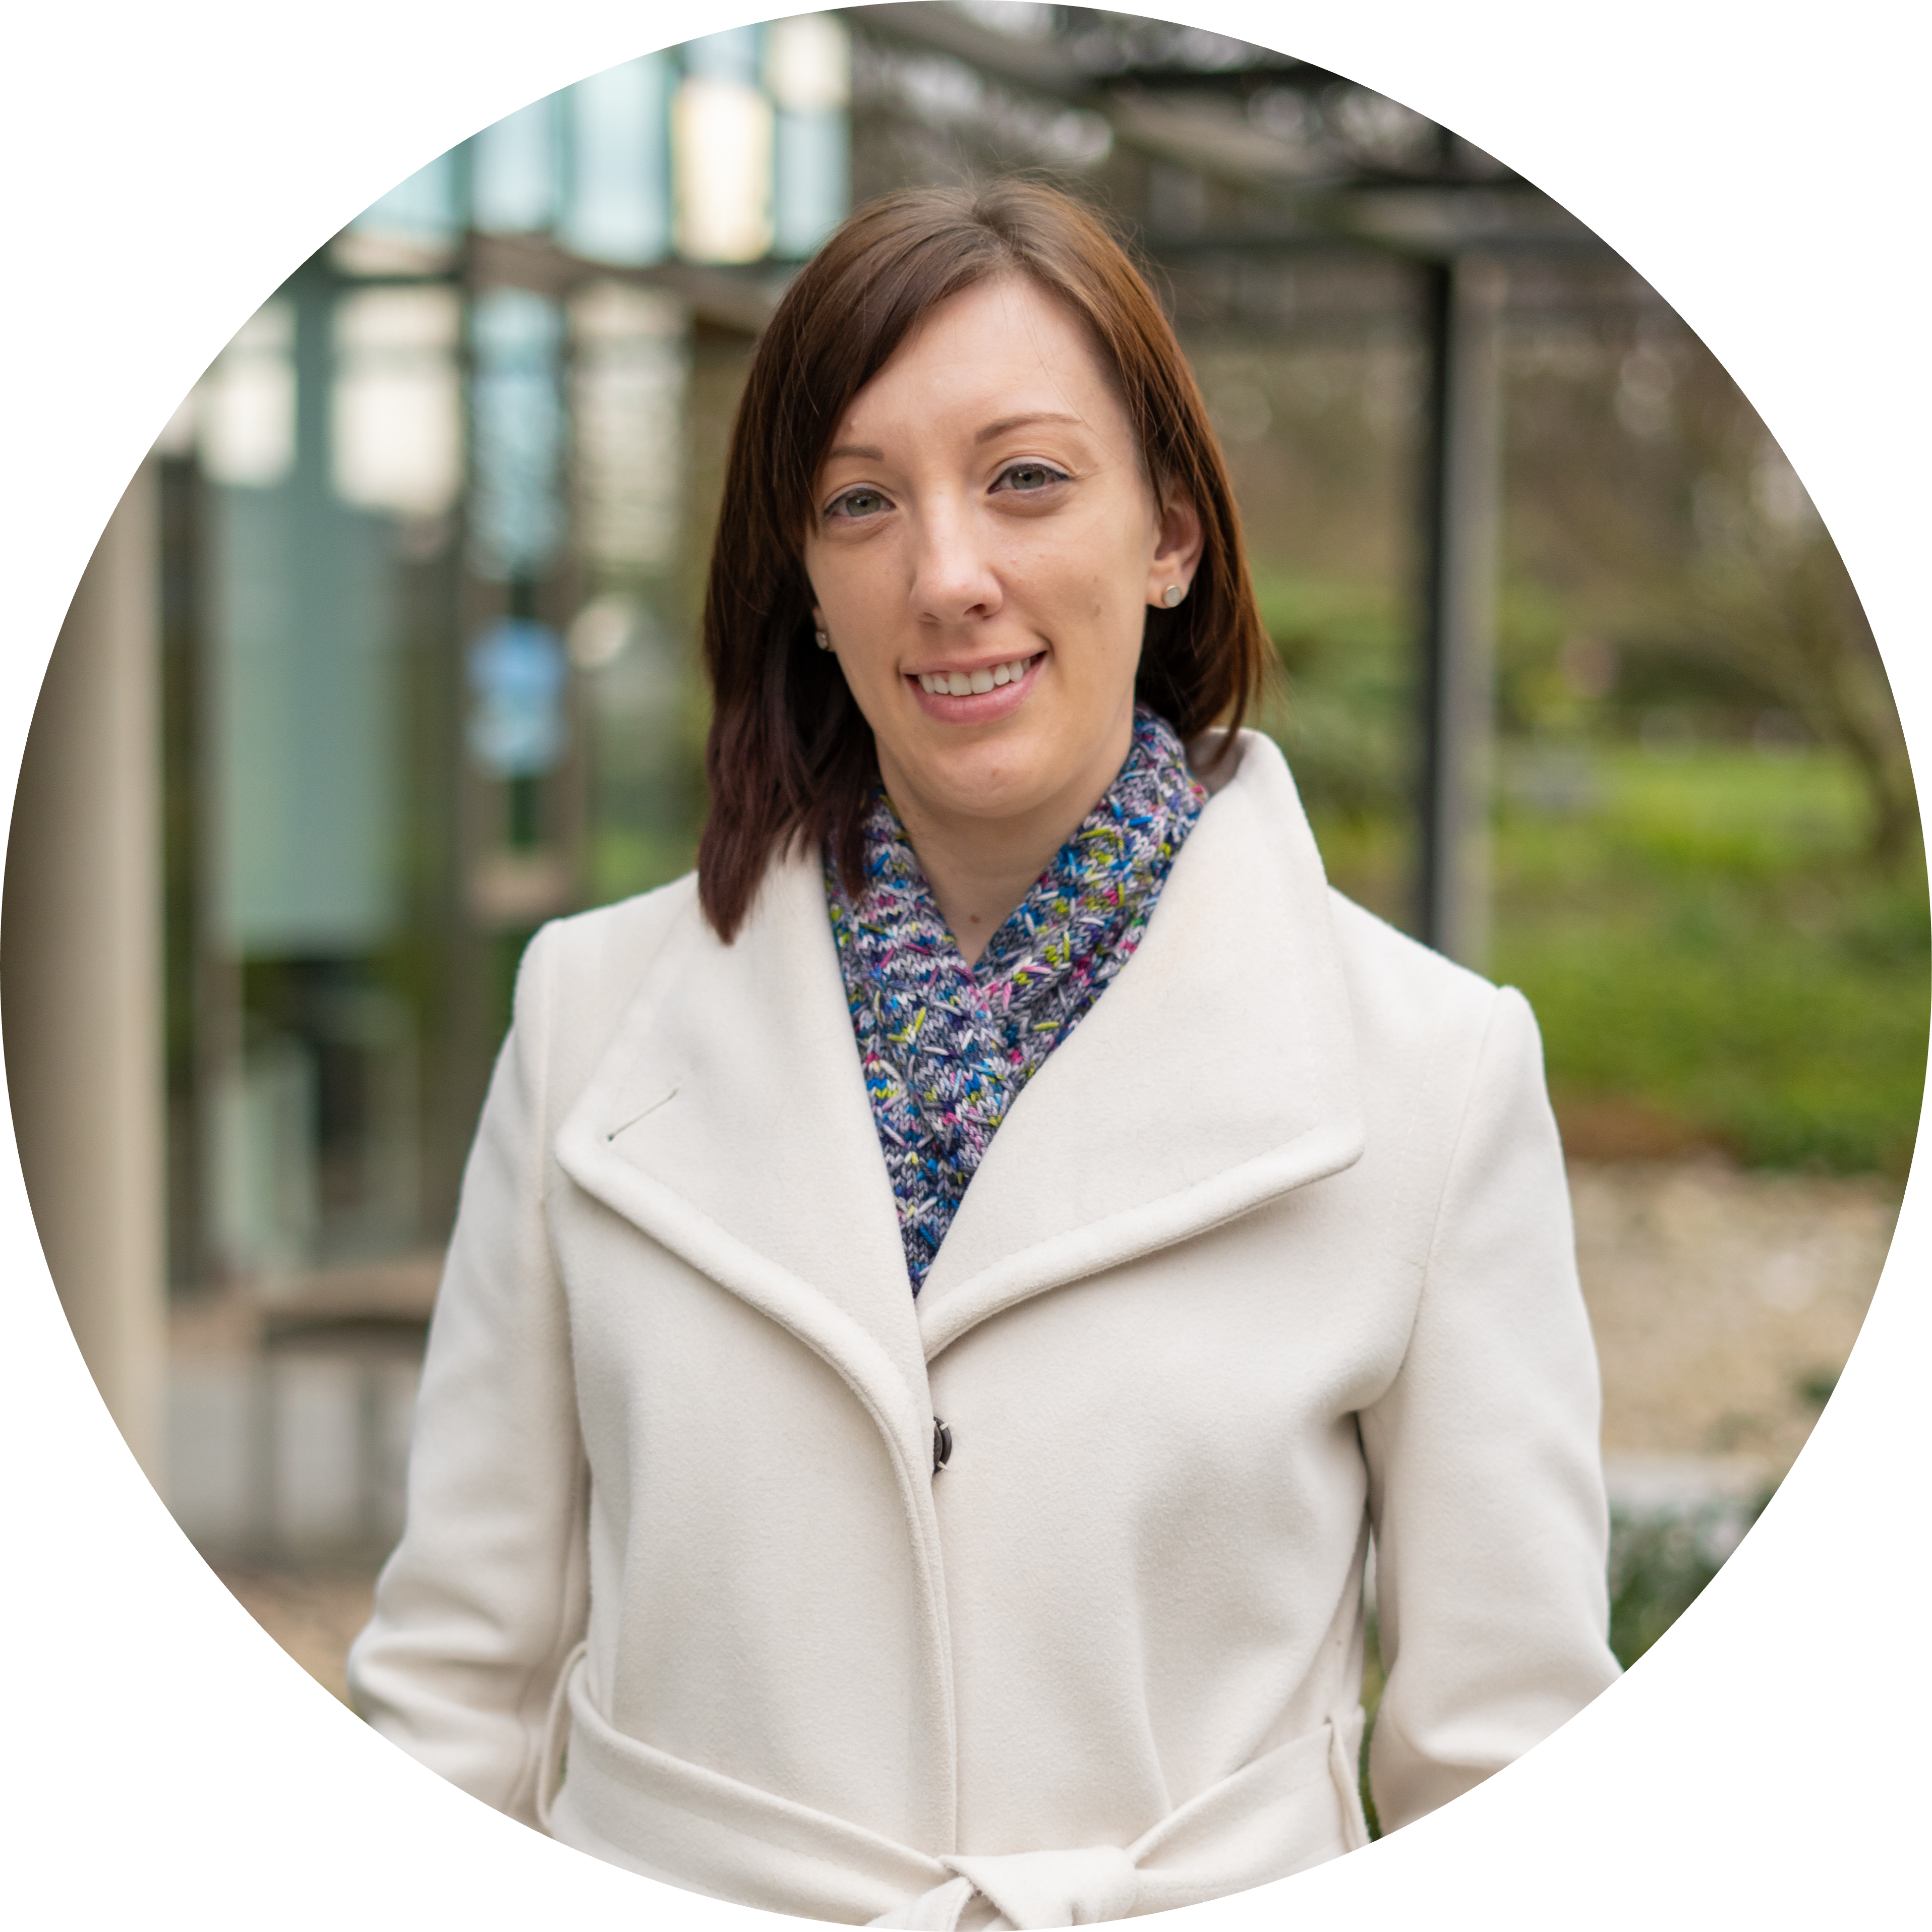
\includegraphics[scale=0.02]{headshot-circle.png} % No idea on how to position this
%\end{figure}

%\setlength{\columnsep}{0pt}
%\begin{wrapfigure}{r}{0cm}
%  \centering
%  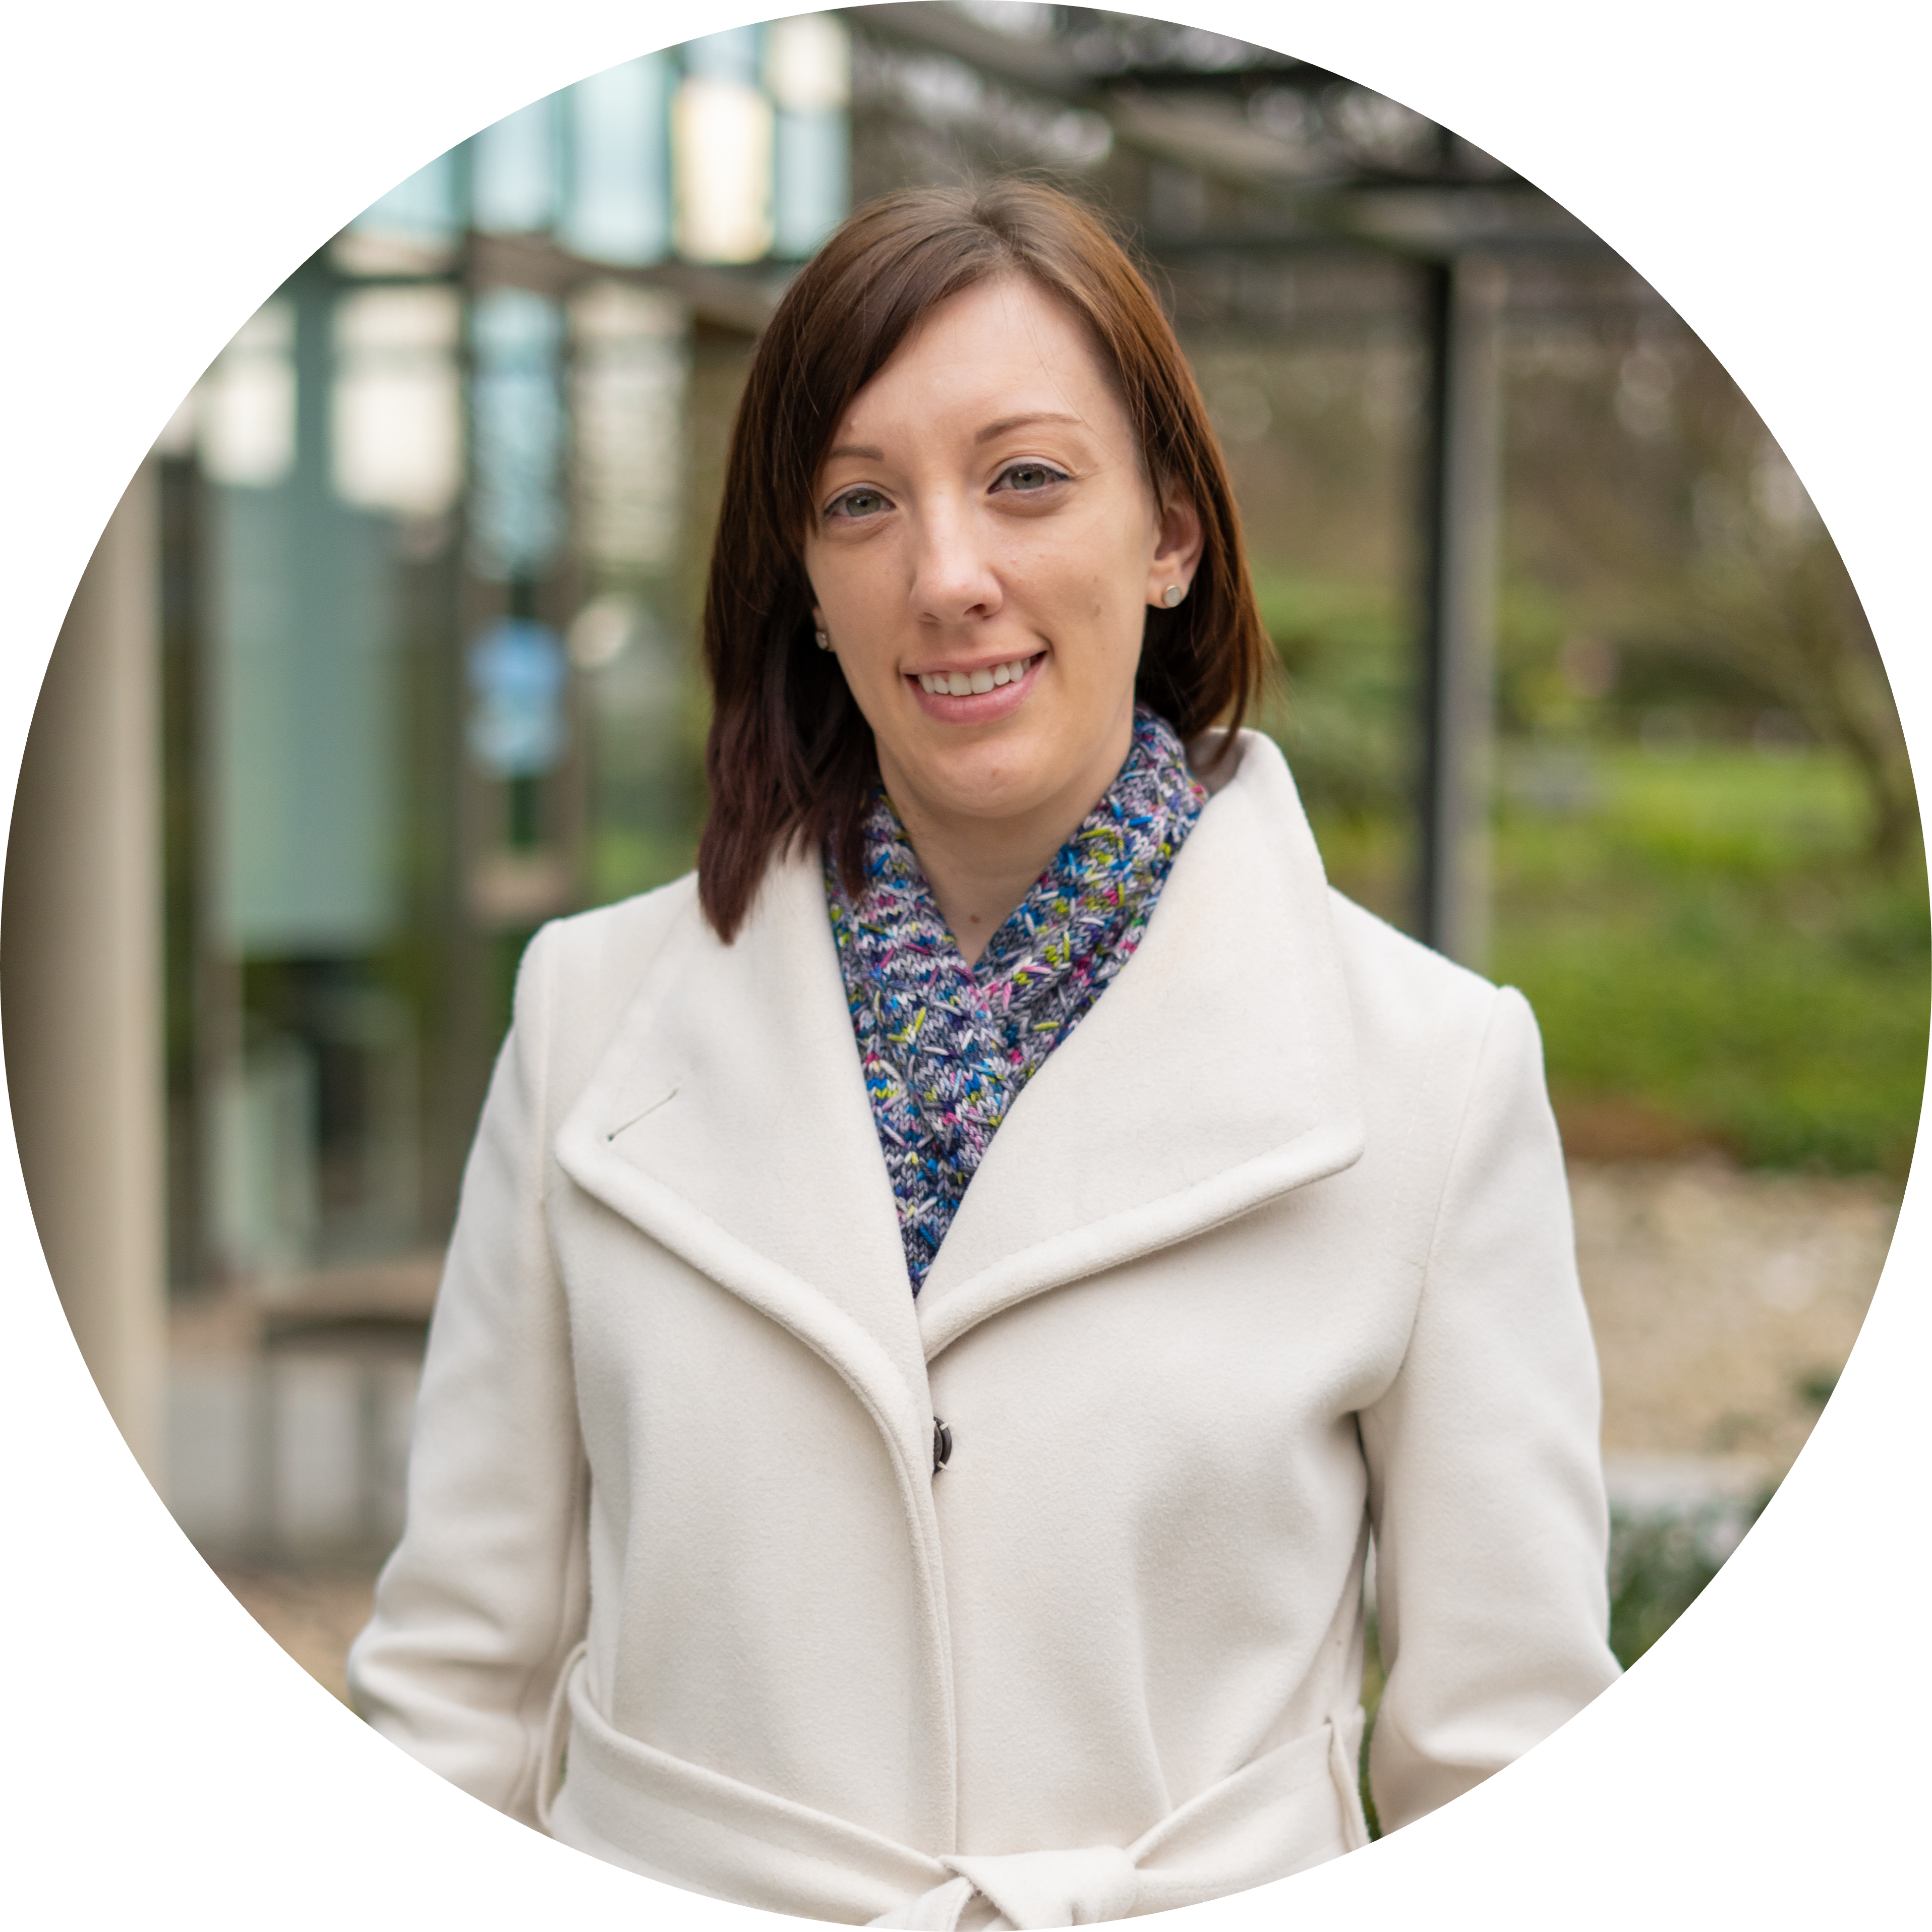
\includegraphics[width=0.2\linewidth]{headshot-circle.png}
%\end{wrapfigure}

%\begin{figure}[t!]
%  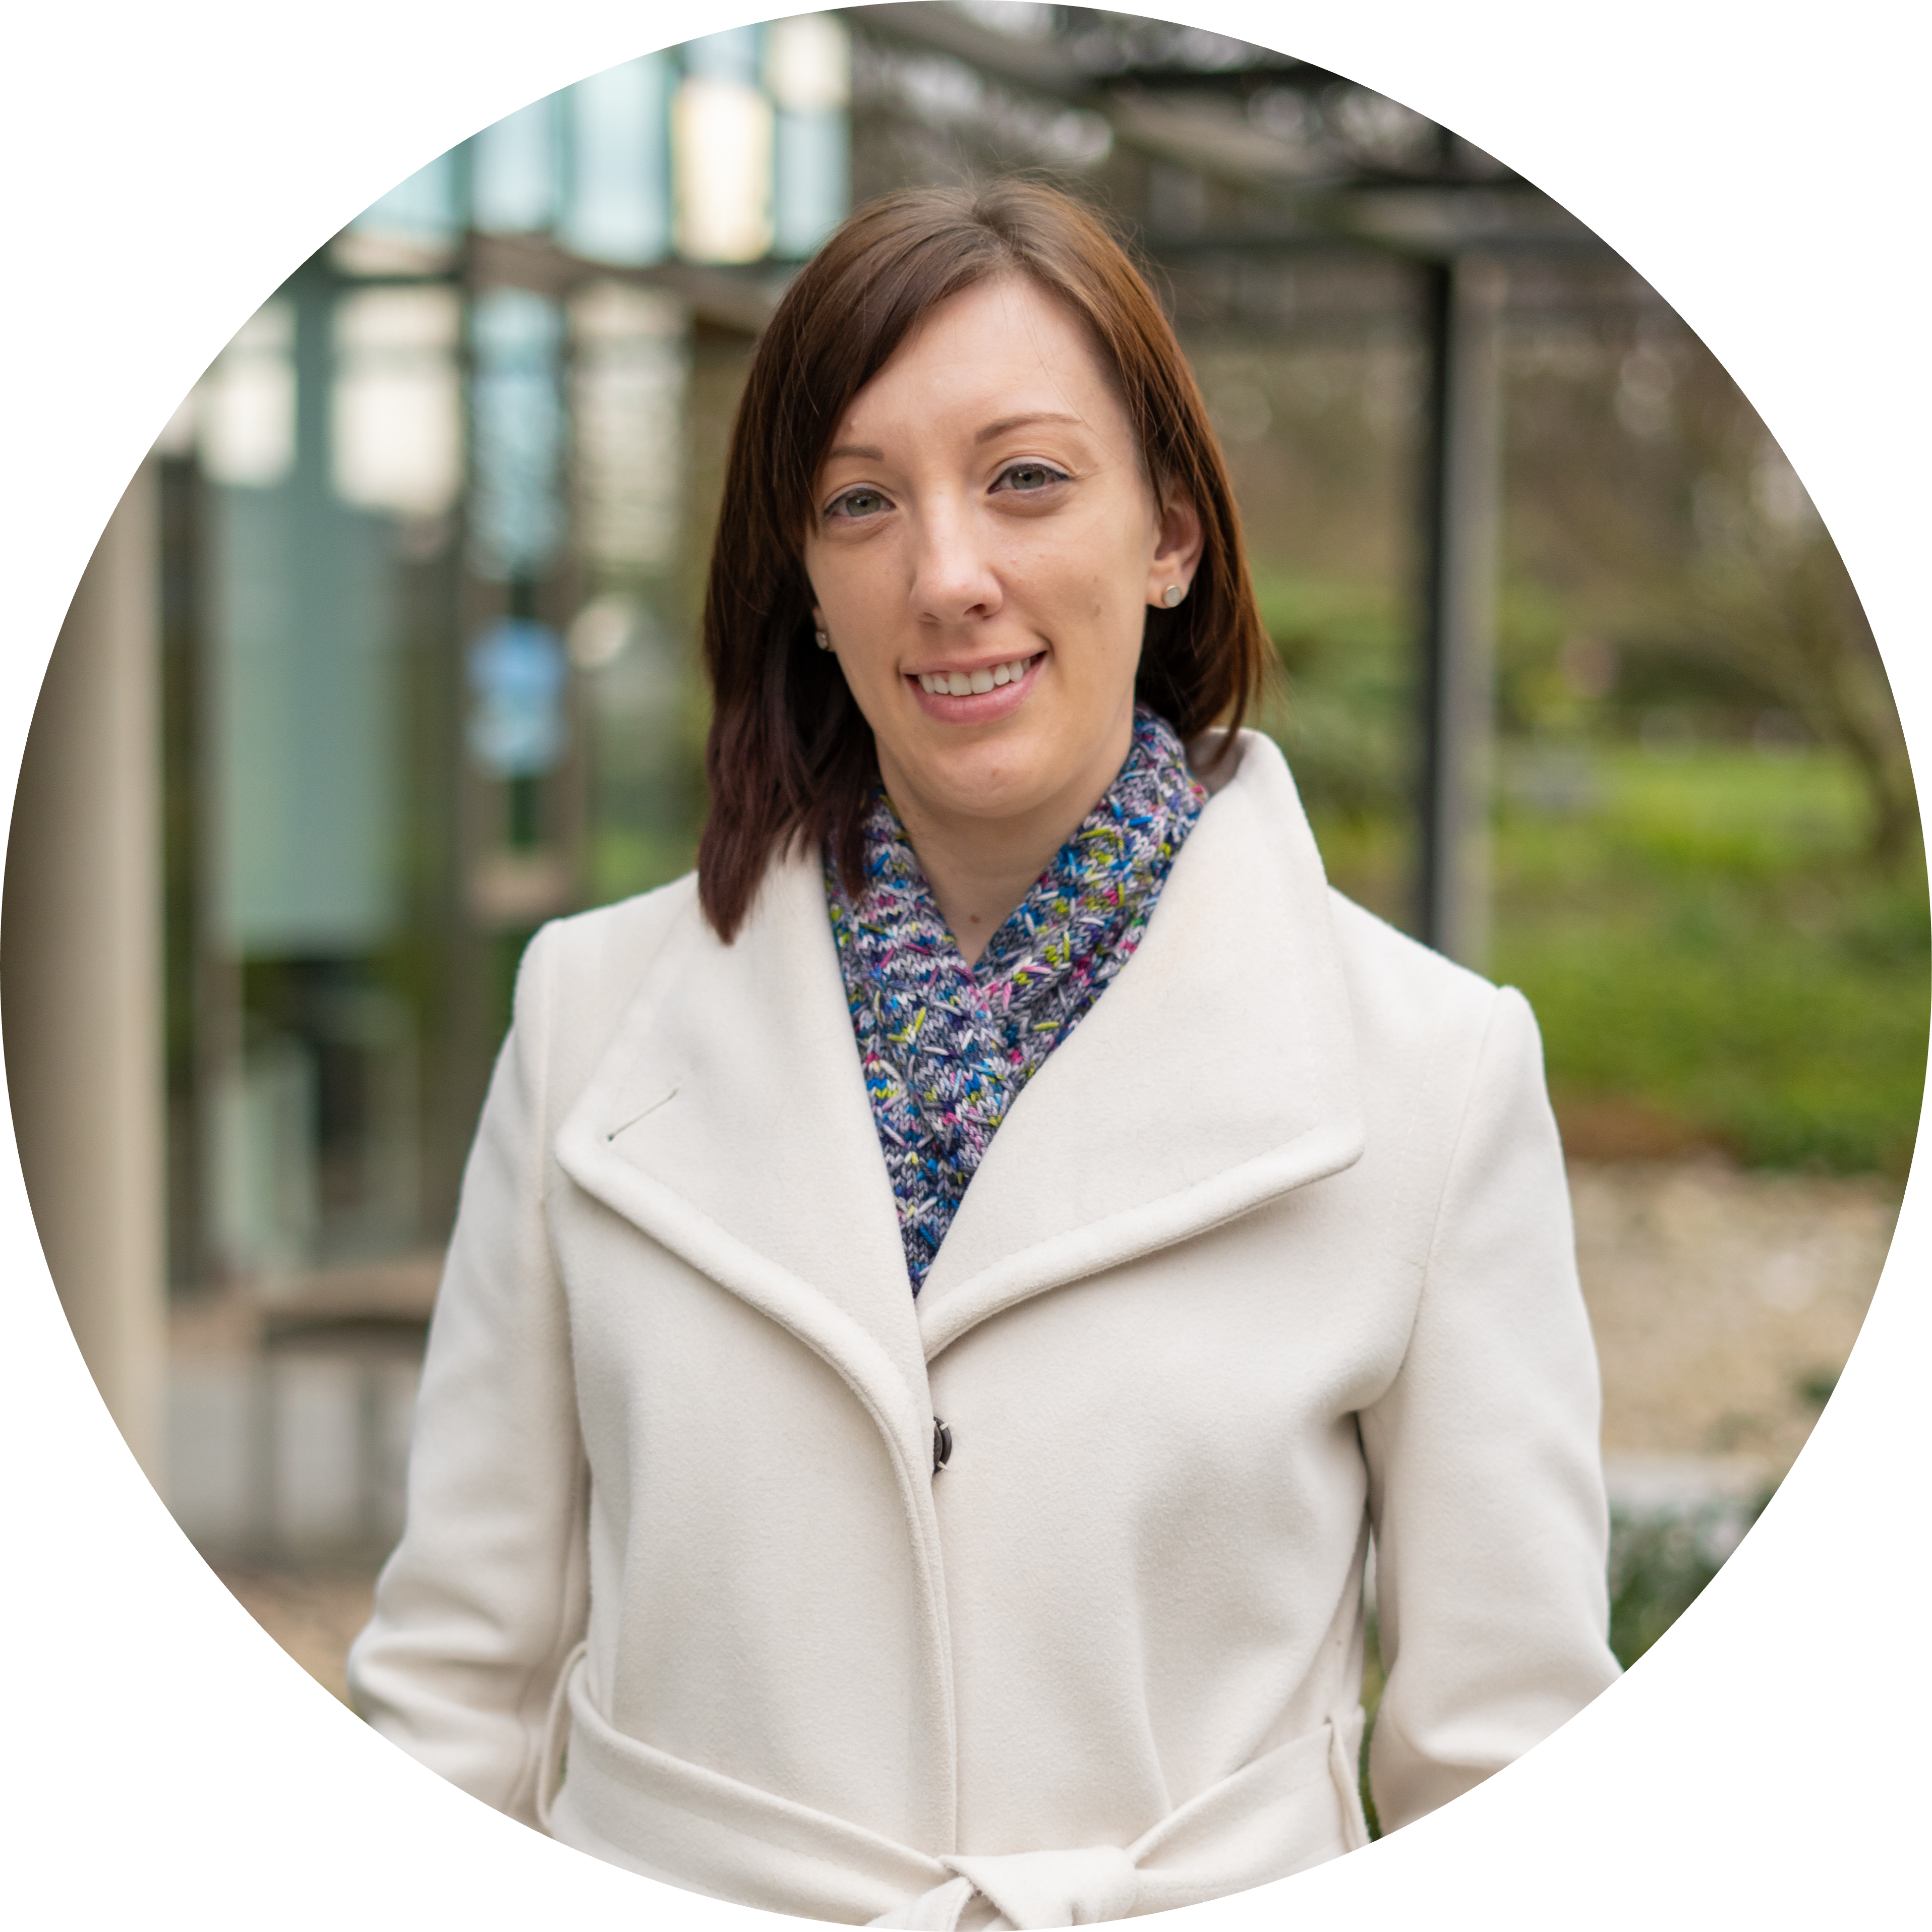
\includegraphics[width=0.15\linewidth]{headshot-circle.png}
%  \label{fig:boat1}
%\end{figure}

\begin{resume}

\section{\sc Who I Am}
Community Builder. Data Sharing Expert. Bioinformatics \& Metadata Enthusiast. Open Science Advocate.
%Community \& Collaboration Builder | Human Data Sharing Expert | Bioinformatics \& Metadata Enthusiast | Open Science Advocate

\section{\sc Contact}
\begin{tabular}{@{}p{3in}p{3in}} %width of columns
{\it Address:} Wellcome Trust Genome Campus & {\em LinkedIn}: \href{https://www.linkedin.com/in/mallory-freeberg/}{\textcolor{blue}{mallory-freeberg}} \\
%{\it Address:} Wellcome Trust Genome Campus & {\em Twitter}: \href{https://twitter.com/MalloryFreeberg}{\textcolor{blue}{@MalloryFreeberg}} \\
{\em Email:}  mallory.freeberg@gmail.com & {\em ORCID:} \href{https://orcid.org/0000-0003-2949-3921}{\textcolor{blue}{0000-0003-2949-3921}} \\
{} & {\em Website:} \href{https://malloryfreeberg.github.io/whoami/}{\textcolor{blue}{malloryfreeberg.github.io/whoami}} \\
\end{tabular}
% {\em Pronouns:} she/her
%Hinxton, Cambridgeshire, CB10 1SD, UK

%\section{\sc Research Interests}
%Genomics/genetics; post-transcriptional gene regulation; high-throughput technologies; second- and third-generation sequencing; data sharing and reuse; open-source tools and platforms enabling life sciences research

\section{\sc Professional Experience}
{\bf EMBL European Bioinformatics Institute}, Cambridge, UK\\
{\em Coordinator}, European Genome-phenome Archive \hfill {Jun 2021 - present}
\begin{itemize}
\itemsep0em 
	\item Contribute expertise to help establish the Federated EGA Network for transnational discovery of and access to sensitive human data
	\item Engage with external partners and stakeholders to ensure data submission, discovery, and distribution services align with community standards
	\item Manage 12-person team responsible for operating production data archive services (\href{https://doi.org/10.1093/nar/gkab1059}{\textcolor{blue}{publication}})
\end{itemize}

{\em UK Biobank Project Lead}, European Genome-phenome Archive \hfill {Aug 2019 - May 2021}
\begin{itemize}
\itemsep0em 
	\item Oversaw data flow to archive 500,000 whole human genomes (12PB of data)
	\item Built and led 3-person team to successfully distribute 4PB of data to cloud-based analysis platform
\end{itemize}

{\em Senior Bioinformatician}, Human Cell Atlas Data Coordination Platform \hfill {Oct 2017 - Jul 2019}
\begin{itemize}
\itemsep0em 
	\item Coordinated data wrangling tasks and priorities for 6-person team across two institutions
	\item Performed curation and ingestion of flagship HCA datasets
	\item Developed HCA metadata standard for cellular-resolution transcriptomics data (\href{https://doi.org/10.1038/s41587-020-00744-z}{\textcolor{blue}{publication}})
	%\item Represented HCA DCP by presenting at three international HCA meetings
\end{itemize}

%{\em Bioinformatician}, Human Cell Atlas Data Coordination Platform \hfill {Oct 2017 - Sep 2018}
%\begin{itemize}
%\itemsep0em 
%	\item Performed curation and ingestion of three flagship HCA datasets
%	\item Developed HCA metadata standard for cellular-resolution transcriptomics data (\href{https://doi.org/10.1038/s41587-020-00744-z}{publication})
%\end{itemize}

{\bf Johns Hopkins University}, Baltimore, MD USA\\
%{\bf The Galaxy Project}, Baltimore, MD USA\\
{\em Trainer}, Galaxy Training Network, The Galaxy Project \hfill {Jan 2017 - Sep 2017}
\begin{itemize}
\itemsep0em 
	\item Designed and delivered seven Galaxy training workshops in three countries (\href{https://doi.org/10.1016/j.cels.2018.05.012}{\textcolor{blue}{publication}})
	\item Created training materials and computational workflows to support reproducible transcriptomics research (\href{https://training.galaxyproject.org/training-material/hall-of-fame/malloryfreeberg/}{\textcolor{blue}{contributions}})
\end{itemize}

{\em Postdoctoral Research Fellow}, Department of Biology \hfill {Jun 2015 - Sep 2017}
\begin{itemize}
\itemsep0em 
	\item Investigated post-transcriptional gene regulatory networks using neural networks
	\item Piloted Oxford Nanopore direct RNA sequencing protocols to catalog transcriptomes
\end{itemize}

%Advisor:  Dr. James Taylor

%{\bf University of Michigan}, Ann Arbor, MI USA\\
%{\em Graduate Student} \hfill {Jul 2009 - May 2015}\\
%Dissertation: Computational analysis of the post-transcriptional gene regulatory network\\
%Advisor:  Dr. John K. Kim

%{\bf Saint Vincent College}, Latrobe, PA USA\\
%{\em Undergraduate Student} \hfill {Jan 2008 - May 2009}\\
%Dissertation: Functional annotation of non-coding elements in the Amphioxus genome\\
%Advisor:  Dr. Michael L. Sierk\\

%{\bf Boyce Thompson Institute for Plant Research}, Ithaca, NY USA\\
%{\em Summer Research Intern} \hfill {May - Aug 2008}\\
%Research: Designed and implemented a motif discovery tool to identify conserved DNA motifs in untranslated gene regions from plants in the {\em Solanaceae} family\\
%Research: Developed computational tool to discover conserved motifs in {\em Solanaceae} genomes\\
%Advisor: Dr. Lukas A. Mueller

%{\bf Johns Hopkins University Applied Physics Laboratory}, Laurel, MD USA\\
%{\em Summer Research Intern} \hfill {May - Aug 2007}\\
%Research: Developed pipeline and built database to identify microorganisms in an environmental sample by comparing mass spectrometry spectral peak data to known protein molecular weights\\
%Research: Designed computational pipeline for microorganism identification by mass spectrometry\\
%Advisors: Drs. Plamen A. Demirev and Richard S. Potember

%{\bf Saint Vincent College}, Latrobe, PA USA\\
%{\em Summer Research Intern} \hfill {May - Aug 2006}\\
%Evaluated the effectiveness of protein databases to classify protein domains using pairwise-, profile-, and structure-based alignment algorithms\\
%Advisor: Dr. Michael L. Sierk

\section{\sc Education}
{\bf PhD Bioinformatics}, University of Michigan, USA \hfill {May 2015}\\
Department of Computational Medicine and Bioinformatics\\ 
Dissertation: Computational analysis of the post-transcriptional gene regulatory network (\href{https://deepblue.lib.umich.edu/bitstream/handle/2027.42/111339/mafree_1.pdf?sequence=1&isAllowed=y}{\textcolor{blue}{thesis}})

{\bf BSc Bioinformatics}, Saint Vincent College, USA \hfill {May 2009}\\
Herbert M. Boyer School of Natural Science, Mathematics, and Computing\\
Dissertation: Functional annotation of non-coding elements in the Amphioxus genome
%{Minors: Biochemistry, Computing/Information Sciences}

\section{\sc Selected Publications}

Corvo A, Matalonga L, Spalding D, {\em et al.} (2023) Remote visualization of large-scale genomic alignments for collaborative clinical research and diagnosis of rare diseases. {\em Cell Genomics}. DOI:\href{https://doi.org/10.1016/j.xgen.2022.100246}{\textcolor{blue}{10.1016/j.xgen.2022.100246}}

Thakur M, Bateman A, Brooksbank C, Freeberg MA, {\em et al.} (2022) EMBL's European Bioinformatics Institute (EMBL-EBI) in 2022. {\em Nucleic Acids Res}. DOI:\href{https://doi.org/10.1093/nar/gkac1098}{\textcolor{blue}{10.1093/nar/gkac1098}}

Freeberg MA, Fromont L, D'Altri T, Romero AF, Ciges JI, Jene A, Kerry G, {\em et al.} (2021) The European Genome-phenome Archive in 2021. {\em Nucleic Acids Res}. DOI:\href{https://doi.org/10.1093/nar/gkab1059}{\textcolor{blue}{10.1093/nar/gkab1059}}

Rehm HL, Page AJH, Smith L, {\em et al.} (2021) GA4GH: International policies and standards for data sharing across genomic research and healthcare. {\em Cell Genomics} 1. DOI:\href{https://doi.org/10.1016/j.xgen.2021.100029}{\textcolor{blue}{10.1016/j.xgen.2021.100029}}

Lawson J, Cabili MN, Kerry G, Boughtwood T, Thorogood A, {\em et al.} (2021) The Data Use Ontology to streamline responsible access to human biomedical datasets. {\em Cell Genomics}.\\ DOI:\href{https://doi.org/10.1016/j.xgen.2021.100028}{\textcolor{blue}{10.1016/j.xgen.2021.100028}}

Füllgrabe A, George N, Green M, Nejad P, {\em et al.} (2020) Guidelines for reporting single-cell RNA-seq experiments. {\em Nat Biotechnol} 38:1384-6. DOI:\href{https://www.nature.com/articles/s41587-020-00744-z}{\textcolor{blue}{10.1038/s41587-020-00744-z}} ({\em arXiv} preprint DOI:\href{https://arxiv.org/abs/1910.14623}{{1910.14623v1}})

%Batut B, Hiltemann S, {\em et al.} (2018) Community-Driven Data Analysis Training for Biology. {\em Cell Syst} 6(6):752-758. DOI:\href{https://doi.org/10.1016/j.cels.2018.05.012}{\textcolor{blue}{10.1016/j.cels.2018.05.012}} ({\em bioRxiv} preprint DOI:\href{https://www.biorxiv.org/content/10.1101/225680v2}{{10.1101/225680}})

\Rightarrow  Full list of publications can be found on \href{https://scholar.google.com/citations?user=2LCcJA0AAAAJ&hl=en}{\textcolor{blue}{Google Scholar}}.

\section{\sc Selected\\ Invited Talks}
%"Title", {\em Conference}; MMM YYYY; City, State/Country (materials)

Federated EGA: Providing global discovery and access for sensitive human data. {\em ISMB/ECCB 2023}; Jul 2023; Lyon, FR (\href{https://docs.google.com/presentation/d/1P9KMd-NAjbz1f9fgO9FVuyYTVAoYZoJAqL0wvnVNrt4/edit?usp=sharing}{\textcolor{blue}{slides}})

The Federated EGA: Global discovery and access for sensitive human data. {\em GA4GH 10th Plenary}; Sep 2022; Barcelona, ES (\href{https://docs.google.com/presentation/d/17wJu5ntPdT1Uj3kSOd_ROHY0DK7IzRwRq6Lgyvso2aw/edit?usp=sharing}{\textcolor{blue}{slides}})

%Sharing sensitive human genomic, phenotypic, and clinical data. {\em Bioinformatics for BioBusiness}; Jul 2022; Manchester, UK (\href{https://docs.google.com/presentation/d/16bB4JdxSbHiNxIqIkVvqjt7rUH4oRMDivPrZRNFp27c/edit?usp=sharing}{\textcolor{blue}{slides}})

FAIR principles and promoting openness in the life sciences. {\em NIHR Statistics Group Workshop}; Feb 2022; virtual (\href{https://docs.google.com/presentation/d/1BNdhj_Ny7qJ84xmoUuzqIicYXF3UwwcGdJTLtyZkV5I/edit?usp=sharing}{\textcolor{blue}{slides}})

The European Genome-phenome Archive Metadata Model. {\em GHGA Workshop on Metadata in Biomedical Genome Research}; Jun 2021; virtual (\href{https://docs.google.com/presentation/d/14x9PNs3j5mNZWIHBW9k6aiJUekiLYsrbrkpaMihB4ko/edit?usp=sharing}{\textcolor{blue}{slides}})

%Human Cell Atlas Data Coordination Platform. {\em Pilot Projects for a Human Cell Atlas Europe Retreat}; Aug 2018; Stockholm, Sweden

%Human Cell Atlas: Google Maps for human anatomy. Cambridge UK Computational Biology and Bioinformatics Meetup; Jun 2018; Cambridge, UK

%Human Cell Atlas Data Coordination Platform Status Update. {\em Human Cell Atlas General Meeting}; Mar 2018; Hinxton, UK (\href{https://youtu.be/NrYH9Oc6Cyk}{\textcolor{blue}{video}})

%Single molecule RNA sequencing of the {\em C. elegans} transcriptome. {\em Molecular Biosystems Conference on Eukaryotic Gene Regulation and Functional Genomics}; Sep 2017; Puerto Varas, CL (\href{https://drive.google.com/file/d/1PKdFgswUhp4K3S_j61xXH5695tnv0Kty/view?usp=sharing}{\textcolor{blue}{slides}})\\
%{\sc Sponsored by Oxford Nanopore Technologies}

%From high school to postdoc: lessons from a decade of bioinformatics education. Great Lakes Bioinformatics Conference; May 2017; University of Illinois at Chicago, Chicago, IL. DOI:10.7490/f1000research.1114161.1

%A novel pipeline for identifying transcriptome-wide binding sites of RNA-binding proteins from PAR-CLIP sequencing data. NCIBI Tools and Technology Seminar Series; May 2013; University of Michigan, Ann Arbor, MI

%Recommendations for successful scientific data sharing: Case studies of next-generation sequencing data use and re-use. NSF Open Data IGERT Seminar; Mar 2013; University of Michigan, Ann Arbor, MI\\

%Defending the genome: Computational identification of germline-specific piRNAs in {\em C. elegans}. Sep 2012; Saint Vincent College, Latrobe, PA

%Next-generation sequencing data re-use facilitates studies of small RNAs. NSF Open Data IGERT Research Workshop; Apr 2012; University of Michigan, Ann Arbor, MI\\

%\Rightarrow  Full list of talks can be found on my \href{https://malloryfreeberg.github.io/whoami/}{\textcolor{blue}{website}}.

\section{\sc Selected\\ Conferences\\ \& Workshops}

%"Title", {\em Conference}; MMM YYYY; City, State/Country (materials)

Demonstrating federated EGA services for sensitive data discovery and access. {\em ELIXIR All Hands 2023}; Jun 2023; Dublin, IE (\href{https://f1000research.com/slides/12-638}{\textcolor{blue}{workshop}})

Resource considerations for establishing and operating a federated human data node. {\em ELIXIR All Hands 2022}; Jun 2022; Amsterdam, NL (\href{https://f1000research.com/posters/11-594}{\textcolor{blue}{poster}})

%Federated EGA Updates in 2022. {\em ELIXIR All Hands 2022}; Jun 2022; Amsterdam, NL (\href{https://f1000research.com/slides/11-623}{\textcolor{blue}{workshop}})

Managing single cell transcriptomics data. {\em EMBL-EBI Training Course}; Jul 2019; Cambridge, UK (\href{https://www.ebi.ac.uk/training/events/managing-single-cell-transcriptomics-data/}{\textcolor{blue}{course}})

%Engaging with the Data Coordination Platform. {\em Human Cell Atlas General Meeting}; May 2019; Tokyo, JP

The Data Coordination Platform: Making the Human Cell Atlas data easily accessible. {\em The Biology of Genomes}; May 2018; Cold Spring Harbor, NY USA (\href{https://drive.google.com/file/d/1KMs4VWE_1rEAFeKLHWrFxHaly5Db78By/view?usp=sharing}{\textcolor{blue}{poster}})

%Approaches for small RNA-seq in Galaxy.{\em Galaxy Community Conference}; Jun 2017; Montpellier, FR (\href{https://doi.org/10.7490/f1000research.1114423.1}{\textcolor{blue}{slides}})

%{\bf Freeberg MA} and Heydarian M. Galaxy 101: A gentle introduction to Galaxy. Galaxy Community Conference; Jun 2017; Montpellier, France (Workshop)

%{\bf Freeberg MA} and Heydarian M. RNAseq analysis in Galaxy. Galaxy Community Conference; Jun 2017; Montpellier, France (Workshop)

%{\bf Freeberg MA} and Heydarian M. Introduction to Genomic Data Analysis with Galaxy. U. S. Food and Drug Administration; Mar 2017; Silver Spring, MD, USA (Workshop)

%{\bf Freeberg MA} and Heydarian M. Introduction to Genomic Data Analysis with Galaxy. Global Biodiversity Genomics Conference; Feb 2017; Washington D.C. (Workshop)

%{\bf Freeberg MA} and Heydarian M. Galaxy to Genomics using NGS Data. 13th KOGO Winter Symposium; Feb 2017; Hongcheon, South Korea (Workshop)

%{\bf Freeberg MA} and Heydarian M. Galaxy to Genomics using NGS Data. Feb 2017; Daejeon and Seoul, South Korea (Workshops)

%{\bf Freeberg MA} and Turaga N. Bioinformagic: Marrying Bioconductor and Galaxy. Galaxy Community Conference; Jun 2016; Bloomington, IN, USA (Workshop)

%{\bf Freeberg MA}. Transcriptome sequencing in nematodes. Oxford Nanopore Technologies London Calling; May 2016; London, UK (Poster)

%{\bf Freeberg MA} and Taylor J. Probabilistic modeling of protein:RNA interaction data identifies functional Transcript States. CSHL Genome Informatics; Oct 2015; Cold Spring Harbor, NY (Poster)

%{\bf Freeberg MA}. Identification and characterization of the mRNA-binding proteome {\em in vivo} in {\em Saccharomyces cerevisiae}. CSHL Systems Biology: Global Regulation of Gene Expression; Mar 2014; Cold Spring Harbor, NY (Talk)

% {\bf Freeberg MA}, Billi AC, and Kim JK. Germline expression, inheritance, and genomic characteristics of {\em Caenorhabditis elegans} 21U-RNAs. 18th International {\em C. elegans} Meeting; Jun 2011; Los Angeles, CA (Poster)

% {\bf Freeberg MA}. Functional Annotation of Non-Coding Elements in the Amphioxus Genome. Saint Vincent College 6th Annual Undergraduate Conference; Apr 2009; Latrobe, PA. (Talk)\\

% {\bf Freeberg MA} and Demirev PA. Bioinformatics Approach to Protein Database Generation for the Identification of Microorganisms by Mass Spectrometry. Saint Vincent College 5th Annual Undergraduate Conference; Apr 2008; Latrobe, PA. (Poster)

% {\bf Freeberg MA} and Sierk ML. Assessment of Homolog Detection by Profile-based Protein Sequence Alignment Methods Against a Structure-based Gold Standard. Duquesne University Annual Summer Undergraduate Research Symposium; Aug 2006; Pittsburgh, PA. (Poster)

%\Rightarrow  Full list of conference and workshop materials can be found on my \href{https://malloryfreeberg.github.io/whoami/}{\textcolor{blue}{website}}.

%\section{\sc Funding} 
%XSEDE Educational Computational Resource Allocation \hfill {2017}\\
%XSEDE Startup Computational Resource Allocation \hfill {2017}\\
%{Galaxy Community Fund, Travel Award (2017)}
%{Rackham Conference Travel Grant (2014)}\\
%Rackham Predoctoral Fellowship \hfill {2013-2014}\\
%NSF Open Data IGERT Fellowship \hfill {2013-2014}\\
%Rackham Graduate Student Research Grant \hfill {2010, 2012}\\
%NIH Bioinformatics Training Grant \hfill {2009-2010}

%\vspace{-.2cm}
%{\bf Saint Vincent College}\\
%{Graduated Summa Cum Laude, 2009}\\
%{President's Award Finalist, 2009}\\
%{Outstanding Bioinformatics Student Award, 2009}
%{Who's Who Among Students in American Universities and Colleges   2009}\\
%{Alpha Lambda Delta Academic Honor Society 2006-2009}

%\section{\sc Computing and Data Analysis Skills} 
%Operating Systems: MacOS X, Linux/Unix \\
%Languages: Python, Perl, SQL, Unix shell \\
%Statistical Packages: R, Bioconductor \\
%Applications: JSON/XML, GitHub, \LaTeX, Galaxy, NGS analysis tools and methodologies\\

%Applications: \LaTeX, MySQL, Galaxy, biomolecule sequence/structure analysis tools, NGS analysis tools and methodologies\\
%Laboratory Techniques: Nanopore sequencing, general molecular biology techniques\\
%Laboratory Techniques: Nanopore sequencing (Oxford Nanopore Technologies), general molecular biology techniques

%\section{\sc Volunteer Activities}
%%{Volunteered for FEMMES Capstone Science weekend}\\
%%{Judged Pioneer High School Science Fair, 2014}\\
%%{Judged Forsythe Middle School Science Fair, 2014}\\
%{Peer reviewed for {\em Cell Rep},  {\em Epigenetics}, {\em Genome Biol}, {\em Genome Res}, {\em PLoS Biol}, {\em RNA}, and {\em RNA Biol} (2013-2014)}\\
%%{Judged Webster Elementary School Science Fair and Exhibition, 2013-2014}\\
%%{Organized departmental happy hours following student seminars, 2012-2014}\\
%{Participated in departmental student recruiting activities, University of Michigan (2011-2015)}\\
%%{Judged Elementary, Middle, and High School Science Fairs, 2013-2014}

\section{\sc Training\\ Courses}

ELIXIR LEadership And Diversity mentoring programme \hfill {2023-present}\\
%Storytelling Workshop \hfill {2021}\\
Managing Managers \hfill {2021}\\
%Moving into Management \hfill {2020}\\
Emotional Intelligence and Mindfulness \hfill {2020}\\
Talented Women's Impact Programme \hfill {2019-2020}\\
EICAT Complementary Scientific Skills Training - Scientific Project Management \hfill {2019}\\
Handling Conflict and Difficult Conversations \hfill {2018}


\section{\sc Teaching \& Mentoring}
{\em Open Life Science}, Cambridge, UK\hfill {Jul 2020 - Present}\\
Mentor, 16-week personal mentorship and cohort-based training program\\
Responsibilities: Mentoring participants on open science practices

{\em STEM Ambassador}, Cambridge, UK\hfill {Jan 2018 - Present}\\
Ambassador, STEM-related public engagement program\\
Responsibilities: Giving talks, demonstrating science experiments, providing career guidance

{\em Johns Hopkins University}, Baltimore, MD USA\hfill {Jan 2017 - May 2017}\\
Instructor, Advanced Academic Program online course: {\em Bioinformatics: Tools for Genome Analysis}\\
Responsibilities: Created course materials, held office hours, graded assignments

%{\bf Sisters Circle}, Baltimore, MD USA\hfill {May 2015 - Sep 2017}\\
%Mentor/tutor for middle school girls\\
%Responsibilities: Co-led weekly after-school sessions, tutored math, mentored 1-on-1

%{\bf University of Michigan}, Ann Arbor, MI USA\hfill {Jul 2014 - Aug 2014}\\
%Mentor for high school student\\
%Responsibilities: Designed bioinformatics/genomics research project, taught shell/perl programming

%{\bf Saint Vincent College}, Latrobe, PA USA\\
%Laboratory Assistant for General Chemistry \hfill { Jan - May 2009}\\
%Responsibilities: Held office hours, prepared and supervised laboratory exercises, graded assignments

%Laboratory Assistant for Genes, Cells, and Computers \hfill { Aug - Dec 2008}\\
%Responsibilities: Held office hours, prepared and supervised laboratory exercises, graded assignments

%Tutor for Bioinformatics, Genomics, and Proteomics \hfill { Aug - Dec 2007}\\
%Responsibilities: Held office hours, led study sessions

\end{resume}
\end{document}

